% Chapter 8: Polyhedra and Euler's Formula
% ch08_polyhedra.tex

\chapter{Polyhedra and Euler's Formula $V - E + F = 2$}

\begin{historical}
In 1752, Euler discovered his famous formula for convex polyhedra: $V - E + F = 2$.
This deceptively simple relationship between vertices, edges, and faces is one of the
most fundamental results in topology. It led to the development of algebraic topology
and the concept of topological invariants. Legendre published the first complete proof
in 1794, and Cauchy gave a simpler proof using projections in 1811. \cite{euler1752}\end{historical}

\section{Euler's Polyhedron Formula}

\begin{theorem}[Euler's Formula]
For any convex polyhedron:
\[
V - E + F = 2
\]
where $V$ = number of vertices, $E$ = number of edges, $F$ = number of faces.
\end{theorem}

\begin{proof}
We prove by induction on the number of faces. For a tetrahedron: $V=4, E=6, F=4$, so $4-6+4=2$.

For the inductive step, remove one face and flatten the remaining polyhedron onto a plane.
This gives a planar graph with the same $V$ and $E$. We can then triangulate all faces by
adding diagonals, which doesn't change $V - E + F$. Finally, remove triangles one at a time
from the outside, each removal preserving $V - E + F$. This leaves a single triangle with
$V=3, E=3, F=2$ (including the outer face), satisfying $3-3+2=2$.
\end{proof}

\begin{lstlisting}[caption={Euler's polyhedron formula}, label=lst:polyhedra]
from euler import euler_polyhedron_formula, platonic_solids, verify_platonic_solids

# Verify Euler's formula for platonic solids
for name, V, E, F in platonic_solids():
    result = euler_polyhedron_formula(V, E, F)
    print(f"{name:12s}: V={V:2d}, E={E:2d}, F={F:2d}, V-E+F={result}")

# Verify all platonic solids
print("\nVerification:")
print(f"  All platonic solids satisfy Euler's formula: {verify_platonic_solids()}")
\end{lstlisting}

\section{The Five Platonic Solids}

\begin{figure}[H]
\centering
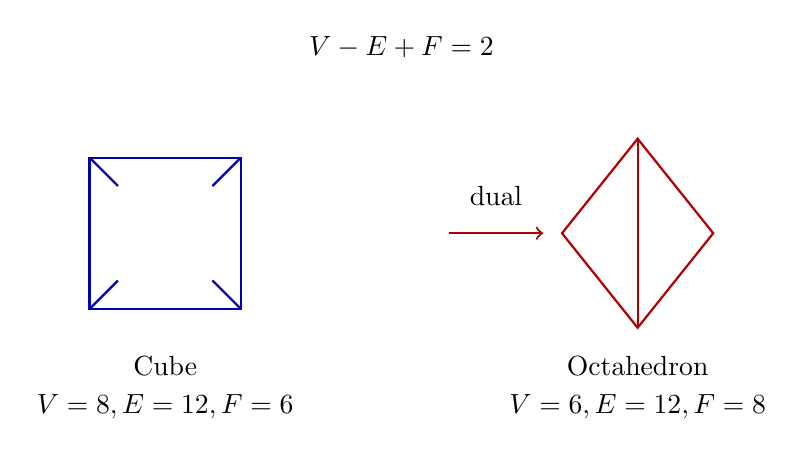
\begin{tikzpicture}[scale=1.2]
  \begin{scope}[shift={(-2.5,0)}]
    \draw[blue!70!black, thick] (-0.8,-0.8) rectangle (0.8,0.8);
    \draw[blue!70!black, thick] (-0.5,-0.5) -- (-0.8,-0.8);
    \draw[blue!70!black, thick] (0.5,-0.5) -- (0.8,-0.8);
    \draw[blue!70!black, thick] (-0.5,0.5) -- (-0.8,0.8);
    \draw[blue!70!black, thick] (0.5,0.5) -- (0.8,0.8);
    \node[below] at (0,-1.2) {Cube};
    \node[below] at (0,-1.6) {$V=8, E=12, F=6$};
  \end{scope}
  \draw[->, thick, red!70!black] (0.5,0) -- (1.5,0);
  \node at (1,0.4) {dual};
  \begin{scope}[shift={(2.5,0)}]
    \draw[red!70!black, thick] (0,-1) -- (0.8,0) -- (0,1) -- (-0.8,0) -- cycle;
    \draw[red!70!black, thick] (0,0) -- (0,-1);
    \draw[red!70!black, thick] (0,0) -- (0,1);
    \node[below] at (0,-1.2) {Octahedron};
    \node[below] at (0,-1.6) {$V=6, E=12, F=8$};
  \end{scope}
  \node[above=0.3cm] at (0,1.5) {$V - E + F = 2$};
\end{tikzpicture}
\caption{Dual relationship: cube $\leftrightarrow$ octahedron}
\label{fig:platonic}
\end{figure}

The five Platonic solids are the only convex polyhedra where all faces are congruent
regular polygons and the same number of faces meet at each vertex.

\begin{table}[H]
\centering
\begin{tabular}{l|c|c|c|c}
Solid & $V$ & $E$ & $F$ & Faces \\
\hline
Tetrahedron & 4 & 6 & 4 & Triangle \\
Cube (Hexahedron) & 8 & 12 & 6 & Square \\
Octahedron & 6 & 12 & 8 & Triangle \\
Dodecahedron & 20 & 30 & 12 & Pentagon \\
Icosahedron & 12 & 30 & 20 & Triangle \\
\end{tabular}
\caption{The five Platonic solids}
\label{tab:platonic}
\end{table}

\begin{theorem}
There are exactly five Platonic solids.
\end{theorem}

\begin{proof}
Let $p$ be the number of edges per face and $q$ be the number of edges meeting at each vertex.
Then $pF = 2E$ and $qV = 2E$. Substituting into Euler's formula:
\[
\frac{2E}{q} - E + \frac{2E}{p} = 2 \implies \frac{1}{p} + \frac{1}{q} = \frac{1}{2} + \frac{1}{E}
\]
Since $p \geq 3$ (minimum for a polygon) and $q \geq 3$ (minimum for a vertex), the only
integer solutions are $(3,3), (3,4), (4,3), (3,5), (5,3)$, corresponding to the five Platonic solids.
\end{proof}

\section{Detailed Properties of Platonic Solids}

\subsection{Geometric Properties}

Each Platonic solid has specific geometric constants:

\begin{table}[H]
\centering
\begin{tabular}{l|c|c|c}
Solid & Dihedral Angle & Vertices per Face & Faces per Vertex \\
\hline
Tetrahedron & $\arccos(1/3) \approx 70.53\circ$ & 3 & 3 \\
Cube & $90\circ$ & 4 & 3 \\
Octahedron & $\arccos(-1/3) \approx 109.47\circ$ & 3 & 4 \\
Dodecahedron & $\arccos(-1/\sqrt{5}) \approx 116.57\circ$ & 5 & 3 \\
Icosahedron & $\arccos(-\sqrt{5}/3) \approx 138.19\circ$ & 3 & 5 \\
\end{tabular}
\caption{Geometric properties of Platonic solids}
\end{table}

\subsection{Schl\"{a}fli Symbols}

The Schl\"{a}fli symbol $\{p,q\}$ denotes a regular polyhedron where each face is a regular $p$-gon
and $q$ faces meet at each vertex. The five Platonic solids have symbols:
$\{3,3\}$, $\{4,3\}$, $\{3,4\}$, $\{5,3\}$, $\{3,5\}$.

\section{Dual Polyhedra}

Every polyhedron has a dual: swap vertices and faces while keeping edges.

\begin{theorem}[Dual Polyhedron]
If a polyhedron has $(V, E, F)$, its dual has $(F, E, V)$.
\end{theorem}

\begin{lstlisting}[caption={Dual polyhedra}, label=lst:dual]
from euler import polyhedron_dual

# Show dual relationships
print("Dual pairs (V,E,F) -> (F,E,V):")
for name, V, E, F in platonic_solids():
    dual_V, dual_E, dual_F = polyhedron_dual(V, E, F)
    print(f"  {name:12s}: ({V}, {E}, {F}) -> ({dual_V}, {dual_E}, {dual_F})")
\end{lstlisting}

The dual relationships are:
\begin{itemize}
\item Tetrahedron is self-dual
\item Cube $\leftrightarrow$ Octahedron
\item Dodecahedron $\leftrightarrow$ Icosahedron
\end{itemize}

\section{Archimedean Solids}

The 13 Archimedean solids are semi-regular convex polyhedra where:
\begin{itemize}
\item All vertices are identical (vertex-transitive)
\item Faces are regular polygons (not all the same)
\item The same sequence of faces appears at each vertex
\end{itemize}

\begin{table}[H]
\centering
\small
\begin{tabular}{l|c|c|c|c}
Solid & $V$ & $E$ & $F$ & Vertex Configuration \\
\hline
Truncated Tetrahedron & 12 & 18 & 8 & 3.6.6 \\
Cuboctahedron & 12 & 24 & 14 & 3.4.3.4 \\
Truncated Cube & 24 & 36 & 14 & 3.8.8 \\
Truncated Octahedron & 24 & 36 & 14 & 4.6.6 \\
Rhombicuboctahedron & 24 & 48 & 26 & 3.4.4.4 \\
Snub Cube & 24 & 60 & 38 & 3.3.3.3.4 \\
Icosidodecahedron & 30 & 60 & 32 & 3.5.3.5 \\
Truncated Dodecahedron & 60 & 90 & 32 & 3.10.10 \\
Truncated Icosahedron & 60 & 90 & 32 & 5.6.6 \\
Rhombicosidodecahedron & 60 & 120 & 62 & 3.4.5.4 \\
Truncated Icosidodecahedron & 120 & 180 & 62 & 4.6.10 \\
Snub Dodecahedron & 60 & 150 & 92 & 3.3.3.3.5 \\
\end{tabular}
\caption{The 13 Archimedean solids}
\label{tab:archimedean}
\end{table}

\section{Topological Invariants}

Euler's formula introduced the concept of a \textbf{topological invariant}: a quantity
unchanged under continuous deformation. The Euler characteristic $\chi = V - E + F$ is
one of the most important topological invariants.

\subsection{Betti Numbers}

The Betti numbers $b_k$ count the number of $k$-dimensional holes in a space:
\begin{itemize}
\item $b_0$: number of connected components
\item $b_1$: number of 1-dimensional holes (cycles)
\item $b_2$: number of 2-dimensional cavities
\end{itemize}

The Euler characteristic can be expressed as the alternating sum of Betti numbers:
\[
\chi = b_0 - b_1 + b_2 - \cdots
\]

For a sphere: $b_0 = 1$, $b_1 = 0$, $b_2 = 1$, so $\chi = 1 - 0 + 1 = 2$.
For a torus: $b_0 = 1$, $b_1 = 2$, $b_2 = 1$, so $\chi = 1 - 2 + 1 = 0$.

\subsection{Homology Groups}

The homology groups $H_k(X)$ provide more refined topological information than Betti numbers.
For a convex polyhedron (homeomorphic to a sphere):
\begin{itemize}
\item $H_0(X) \cong \mathbb{Z}$ (connected)
\item $H_1(X) \cong 0$ (simply connected)
\item $H_2(X) \cong \mathbb{Z}$ (encloses a 2-dimensional cavity)
\end{itemize}

\section{Generalization: Surfaces of Higher Genus}

Euler's formula generalizes to surfaces with holes (genus $g$):
\[
V - E + F = 2 - 2g
\]

\begin{itemize}
\item Sphere: $g = 0$, so $V - E + F = 2$
\item Torus: $g = 1$, so $V - E + F = 0$
\item Double torus: $g = 2$, so $V - E + F = -2$
\end{itemize}

\begin{lstlisting}[caption={Euler characteristic for surfaces}, label=lst:genus]
from euler import euler_characteristic_genus

print("Euler characteristic for surfaces of genus g:")
for g in range(4):
    V, E, F = 2 - 2*g, 0, 0  # placeholder
    print(f"  Genus {g}: \chi = {2 - 2*g}")
\end{lstlisting}

\section{Cayley's Formula for Trees}

A fundamental result in graph theory states that the number of labeled trees on $n$ vertices
is $n^{n-2}$ (Cayley's formula, 1889).

\begin{theorem}[Cayley's Formula]
The number of distinct labeled trees on $n$ vertices is $n^{n-2}$.
\end{theorem}

\begin{proof}
One proof uses Pr\"{u}fer sequences: every labeled tree on $n$ vertices corresponds uniquely
to a sequence of length $n-2$ with elements from $\{1, 2, \ldots, n\}$. There are $n^{n-2}$
such sequences.
\end{proof}

\section{Eigenvalue Analysis of Polyhedral Graphs}

The adjacency matrix of a polyhedral graph (1-skeleton of a convex polyhedron) has
important spectral properties:

\begin{theorem}
For a $d$-regular polyhedral graph with $n$ vertices and adjacency matrix $A$:
\begin{itemize}
\item $\lambda_1 = d$ (the degree)
\item $\lambda_2 > -1$ (the graph is an expander)
\item The graph is connected iff $\lambda_1 > \lambda_2$
\end{itemize}
\end{theorem}

\begin{lstlisting}[caption={Eigenvalue analysis of polyhedral graphs}, label=lst:eigenvalue_poly]
import numpy as np
from scipy.linalg import eigvals

# Adjacency matrix of a cube graph
A_cube = np.array([
    [0,1,1,0,1,0,0,0],
    [1,0,0,1,0,1,0,0],
    [1,0,0,1,0,0,1,0],
    [0,1,1,0,0,0,0,1],
    [1,0,0,0,0,1,1,0],
    [0,1,0,0,1,0,0,1],
    [0,0,1,0,1,0,0,1],
    [0,0,0,1,0,1,1,0]
])

eigenvalues = eigvals(A_cube)
print(f"Cube eigenvalues: {np.sort(eigenvalues)[::-1].real}")
print(f"Largest eigenvalue: {np.max(eigenvalues.real):.2f} (should be 3)")
\end{lstlisting}

\section{Applications}

\begin{itemize}
\item \textbf{Network theory:} Relating nodes, connections, and regions
\item \textbf{Chemistry:} Analyzing molecular structures (fullerenes, carbon nanotubes)
\item \textbf{Computer graphics:} Mesh validation and error detection
\item \textbf{Topology:} Classifying surfaces by genus
\item \textbf{Crystallography:} Understanding crystal structures
\item \textbf{Voronoi diagrams:} Dual relationships with Delaunay triangulations
\end{itemize}

\section{Computational Complexity}

\subsection{Verifying Euler's Formula}
\begin{itemize}
\item Input: $(V, E, F)$ tuple
\item Time: $O(1)$ arithmetic operations
\item Space: $O(1)$
\end{itemize}

\subsection{Finding Euler Characteristic}
\begin{itemize}
\item From graph traversal: $O(V + E)$ for planar graphs
\item From topological data analysis: $O(n^2)$ for general complexes
\end{itemize}

\section{Frequently Asked Questions}

\begin{itemize}
\item \textbf{Q: Why does Euler's formula only work for convex polyhedra?} \\
The formula holds for any polyhedron homeomorphic to a sphere. Non-convex polyhedra with holes (like a toroidal polyhedron) have a different Euler characteristic. The key requirement is that the polyhedron can be continuously deformed into a sphere without tearing.

\item \textbf{Q: What is the Euler characteristic?} \\
The Euler characteristic $\chi = V - E + F$ is a topological invariant. For a sphere it's 2, for a torus it's 0, and for a surface of genus $g$ it's $2 - 2g$. It classifies surfaces up to homeomorphism.

\item \textbf{Q: How does Euler's formula relate to the Four Color Theorem?} \\
Euler's formula is a key ingredient in the proof of the Four Color Theorem. It helps establish that every planar graph has a vertex of degree at most 5, which is used in the discharging method.

\item \textbf{Q: Can Euler's formula be used for non-polyhedral surfaces?} \\
Yes, by triangulating the surface. Any compact surface can be triangulated, and the Euler characteristic is independent of the triangulation.

\item \textbf{Q: What is the dual of a cube?} \\
The dual of a cube is an octahedron: each face becomes a vertex and each vertex becomes a face. The cube has 6 faces and 8 vertices; the octahedron has 8 faces and 6 vertices.

\item \textbf{Q: How do fullerenes relate to Euler's formula?} \\
Fullerenes (carbon molecules like C60) are polyhedra with only pentagonal and hexagonal faces. Euler's formula forces exactly 12 pentagons in any such structure, regardless of the number of hexagons.

\item \textbf{Q: What is the significance of the Euler characteristic in physics?} \\
The Euler characteristic appears in the Gauss-Bonnet theorem, relating the geometry of a surface to its topology. In condensed matter physics, it appears in the study of band structures and topological insulators.

\item \textbf{Q: What are Betti numbers?} \\
Betti numbers $b_k$ count the number of $k$-dimensional holes in a topological space. The Euler characteristic is the alternating sum $\chi = b_0 - b_1 + b_2 - \cdots$.

\item \textbf{Q: How does the spectral gap relate to graph connectivity?} \\
For a $d$-regular graph, the spectral gap $d - \lambda_2$ measures expansion properties. A large spectral gap indicates good connectivity and fast mixing of random walks.
\end{itemize}

\section{Exercises}

\begin{exercise}
Prove Euler's formula for the cube by direct counting.
\end{exercise}

\begin{exercise}
Show that the dodecahedron and icosahedron are duals of each other.
\end{exercise}

\begin{exercise}
Prove that every planar graph has a vertex of degree at most 5 using Euler's formula.
\end{exercise}

\begin{exercise}[Computational]
Implement a function that verifies Euler's formula for arbitrary polyhedra given their vertex, edge, and face lists.
\end{exercise}

\begin{exercise}
Calculate the Euler characteristic of a torus using a square with opposite sides identified.
\end{exercise}

\begin{exercise}
Show that any polyhedron made only of hexagons and pentagons (like a soccer ball) must have exactly 12 pentagons.
\end{exercise}

\begin{exercise}
Prove that the sum of angles in a spherical triangle exceeds $\pi$ radians, and relate this to the Euler characteristic of the sphere.
\end{exercise}

\begin{exercise}
Show that a convex polyhedron with all faces being triangles satisfies $E = 3V - 6$ and $F = 2V - 4$.
\end{exercise}

\begin{exercise}
Verify that all 13 Archimedean solids satisfy Euler's formula $V - E + F = 2$.
\end{exercise}

\begin{exercise}[Computational]
Compute the eigenvalues of the adjacency matrices for all five Platonic solids and verify that the largest eigenvalue equals the vertex degree.
\end{exercise}

\begin{exercise}
Prove that the number of labeled trees on $n$ vertices is $n^{n-2}$ using Pr\"{u}fer sequences.
\end{exercise}

\begin{exercise}
Show that the complete graph $K_5$ is non-planar by proving it violates the inequality $E \leq 3V - 6$.
\end{exercise}

\begin{exercise}
Calculate the Betti numbers for the surface of a torus and verify that $\chi = 0$.
\end{exercise}

\begin{exercise}
Prove that the dual of an Archimedean solid is a Catalan solid.
\end{exercise}

\begin{exercise}[Computational]
Implement a function to compute the Euler characteristic of a simplicial complex from its vertex, edge, and face lists.
\end{exercise}
